\documentclass[12pt,a4paper]{article}
\usepackage[UTF8]{ctex}
\usepackage{amsmath,amssymb}
\usepackage{graphicx}
\usepackage{booktabs}
\usepackage{longtable}
\usepackage{array}
\usepackage{listings}
\usepackage{xcolor}
\usepackage{geometry}
\usepackage{float}
\usepackage{hyperref}
\usepackage{cite}
\usepackage{subcaption}
\usepackage{pdfpages}

\geometry{margin=2.5cm}

% 代码样式设置
\lstset{
    basicstyle=\ttfamily\small,
    keywordstyle=\color{blue},
    commentstyle=\color{green!50!black},
    stringstyle=\color{red},
    numberstyle=\tiny\color{gray},
    frame=single,
    breaklines=true,
    showstringspaces=false,
    numbers=left,
    numbersep=5pt,
    tabsize=4
}

\title{基于机器学习的金融市场欺骗交易检测系统\thanks{代码地址: \url{https://github.com/fenglang918/Spoofing-Detect}}}
\author{冯亮 24210680035}
\date{\today}

\begin{document}

% 插入封面页

\includepdf[pages=1]{封面.pdf}
\newpage

\maketitle

\begin{abstract}
金融市场中的欺骗交易(Spoofing)是一种通过虚假委托单操纵价格的市场操纵行为,严重损害了市场的公平性和效率。本文提出了一个基于机器学习的端到端欺骗交易检测系统,专门针对中国A股市场的高频交易数据进行分析。系统采用多层次的数据处理流程,包括原始数据清洗、特征工程、标签生成和模型训练等模块。在标签生成方面,我们设计了基于时间窗口和价格偏离的复合规则,结合扩展的行为模式识别算法,生成高质量的训练标签。特征工程模块提取了29个维度的交易特征,涵盖价格、数量、时间、技术指标和统计特征等多个方面。模型训练采用集成学习方法,结合LightGBM、XGBoost和随机森林算法,并通过Focal Loss和类别权重等技术处理数据不平衡问题。在包含近300万训练样本和89万验证样本的大规模数据集上,系统达到了ROC-AUC 0.782和PR-AUC 0.032的性能,且在预测概率最高的0.5\%样本中精确率(Precision@0.5\%)达到了7.32\%,在极度不平衡的数据分布下(正样本比例仅0.71\%)展现了良好的检测能力。本研究为金融监管机构提供了一个实用的技术工具,对维护市场公平和投资者利益具有重要意义。

\textbf{关键词:} 欺骗交易检测;机器学习;高频交易;市场操纵;集成学习
\end{abstract}

\section{引言}

金融市场的健康发展是现代经济体系的重要基石,而市场操纵行为则是威胁市场公平性和效率的重要因素。欺骗交易(Spoofing)作为一种典型的市场操纵手段,通过大量虚假委托单的快速提交和撤销来误导其他投资者,从而操纵股价并获取非法利润。随着电子交易系统的普及和高频交易技术的发展,这种操纵行为变得更加隐蔽和复杂,给监管机构带来了巨大挑战。

近年来,机器学习技术在金融风险管理和异常检测领域得到了广泛应用。相比传统的基于规则的检测方法,机器学习方法能够从大量历史数据中自动学习复杂的模式,提高检测的准确性和效率。然而,将机器学习技术应用于欺骗交易检测仍面临诸多挑战:首先,金融时间序列数据具有高维度、高噪声和非线性等特点;其次,欺骗交易样本极度稀少,导致严重的数据不平衡问题;最后,监管要求的可解释性与机器学习模型的黑盒特性之间存在矛盾。

本文针对上述挑战,设计并实现了一个基于机器学习的端到端欺骗交易检测系统。该系统专门针对中国A股市场的特点,采用了创新的标签生成算法、全面的特征工程方法和先进的集成学习技术。主要贡献包括:

\textbf{(1) 设计了多层次的标签生成机制}:基于R1(快速撤单)和R2(价格操纵)规则的基础标签,结合极端价格偏离、激进定价、异常大单和异常时间段活动等扩展模式,生成更加全面和准确的训练标签。

\textbf{(2) 构建了comprehensive特征工程系统}:提取了包括价格特征、时间特征、订单簿特征、技术指标和统计特征在内的29个维度特征,并采用严格的数据泄露防护机制,确保特征的时效性和可靠性。

\textbf{(3) 实现了robust的集成学习框架}:结合LightGBM、XGBoost和随机森林等多种算法,采用Focal Loss、类别权重和智能采样等技术解决数据不平衡问题,并通过Optuna进行超参数优化。

\textbf{(4) 建立了完整的评估和可视化体系}:设计了针对不平衡数据的评估指标体系,包括PR-AUC、ROC-AUC和Precision@K等指标,并创新性地提出了专门针对极度不平衡数据的可视化方案,解决了传统可视化方法的误导性问题。

实验结果表明,在包含近380万样本的大规模数据集上,本系统在极度不平衡的数据分布下(正样本比例仅0.71\%)达到了ROC-AUC 0.782的良好性能,证明了方法的有效性。

\section{文献综述}

\subsection{欺骗交易的定义与监管现状}

欺骗交易(Spoofing)是指交易者通过提交大量虚假委托单来制造虚假的市场深度或价格趋势,误导其他市场参与者,然后在价格向有利方向移动后撤销虚假委托并执行真实交易的行为\cite{cartea2018algorithmic}。这种行为在全球主要金融市场都被明确禁止,美国商品期货交易委员会(CFTC)在2010年的《多德-弗兰克法案》中首次将其定义为非法行为,欧盟在《市场滥用法规》(MAR)中也有相应规定。

在中国,证监会和交易所也在不断完善相关监管制度。深圳证券交易所在2018年发布的《股票异常交易实时监控细则》中明确规定了对虚假申报等异常交易行为的监控要求。然而,随着算法交易和高频交易的快速发展,传统的基于规则的监控方法已难以应对日益复杂的操纵手段。

\subsection{传统检测方法}

早期的欺骗交易检测主要依赖基于规则的方法。Scopino\cite{scopino2015regulatory}提出了基于委托量比例和撤单时间的简单规则,通过统计分析识别可疑交易行为。Allen和Gale\cite{allen1992stock}从理论角度分析了市场操纵的经济学原理,为后续的检测算法奠定了基础。

Kumar和Seppi\cite{kumar1992futures}针对期货市场设计了基于价格和成交量异常的检测规则。他们发现,真实的欺骗交易往往表现出委托量大、撤单频繁、价格影响显著等特征。这些早期研究为后续的机器学习方法提供了重要的领域知识。

然而,基于规则的方法存在明显局限性:一是规则阈值的设定往往依赖专家经验,缺乏客观性;二是面对复杂多变的操纵策略,静态规则难以适应;三是误报率较高,增加了监管成本。

\subsection{机器学习在金融异常检测中的应用}

近年来,机器学习技术在金融异常检测领域得到了广泛应用。Patel等\cite{patel2015predicting}采用支持向量机(SVM)和随机森林算法检测期货市场的异常交易,取得了较好的效果。Cao等\cite{cao2014detecting}使用深度学习方法分析高频交易数据,识别潜在的市场操纵行为。

在欺骗交易检测的具体应用中,Cartea等\cite{cartea2018algorithmic}提出了基于马尔可夫链的隐含状态模型,通过分析委托单到达和撤销的时间序列模式来识别欺骗行为。Ye等\cite{ye2020machine}采用LSTM神经网络处理时间序列特征,在模拟数据上取得了较高的检测准确率。

但现有研究主要存在以下问题:(1) 大多数研究使用模拟数据或小规模数据集,缺乏大规模真实数据验证;(2) 对于数据不平衡问题的处理不够充分;(3) 特征工程往往不够系统化,缺乏对金融领域知识的深度整合。

\subsection{不平衡数据处理技术}

欺骗交易检测面临的一个核心挑战是数据极度不平衡。在真实市场数据中,欺骗交易样本通常只占总样本的不到1\%,这给传统机器学习算法带来了巨大挑战。

针对不平衡数据问题,主要的解决方案包括:

\textbf{采样技术}:包括随机欠采样、SMOTE过采样等。He和Garcia\cite{he2009learning}对各种采样技术进行了全面比较,发现在极度不平衡的情况下,简单的欠采样往往比复杂的过采样方法更有效。

\textbf{代价敏感学习}:通过调整不同类别的错误分类代价来平衡模型性能。Elkan\cite{elkan2001foundations}提出了代价敏感学习的理论框架,广泛应用于不平衡数据分类问题。

\textbf{集成学习方法}:如AdaBoost、随机森林等,通过组合多个弱分类器来提升性能。Chen和Guestrin\cite{chen2016xgboost}提出的XGBoost算法在处理不平衡数据方面表现优异。

\textbf{新的损失函数}:如Focal Loss,专门针对极度不平衡数据设计。Lin等\cite{lin2017focal}在目标检测任务中首次提出了Focal Loss,后被广泛应用于各种不平衡分类问题。

\section{方法论}

\subsection{系统架构设计}

本文提出的欺骗交易检测系统采用端到端的架构设计,包含数据处理、特征工程、标签生成、模型训练和预测分析五个核心模块,如图\ref{fig:system_architecture}所示。

\begin{table}[H]
\centering
\caption{欺骗交易检测系统架构流程}
\label{fig:system_architecture}
\begin{tabular}{cll}
\toprule
步骤 & 模块名称 & 主要功能 \\
\midrule
1 & 数据处理模块 & 原始交易数据清洗、合并和格式化 \\
2 & 特征工程模块 & 提取价格、数量、时间等多维度特征 \\
3 & 标签生成模块 & 基于R1/R2规则生成欺骗交易标签 \\
4 & 模型训练模块 & 集成学习训练欺骗交易检测模型 \\
5 & 预测分析模块 & 模型预测和可视化分析 \\
\bottomrule
\end{tabular}
\end{table}

\textbf{数据处理模块}负责原始交易数据的清洗、合并和格式化,将来自不同数据源的委托和成交记录整合为统一的事件流格式。

\textbf{特征工程模块}从事件流数据中提取多维度的交易特征,包括价格、数量、时间、技术指标和统计特征等。

\textbf{标签生成模块}基于领域知识和监管规则,为每个委托事件生成是否为欺骗交易的标签。

\textbf{模型训练模块}采用集成学习方法,结合多种机器学习算法训练欺骗交易检测模型。

\textbf{预测分析模块}使用训练好的模型对新的交易数据进行预测,并提供可视化分析结果。

图\ref{fig:system_flow}展示了系统的完整数据流和处理流程:

\begin{figure}[H]
\centering
\fbox{\parbox{0.8\textwidth}{
\centering
\textbf{欺骗交易检测系统数据流程图}
\vspace{0.5cm}

\textbf{数据输入} $\rightarrow$ \textbf{数据清洗} $\rightarrow$ \textbf{特征提取} $\rightarrow$ \textbf{标签生成}

$\downarrow$

\textbf{训练数据集} $\rightarrow$ \textbf{模型训练} $\rightarrow$ \textbf{性能评估}

$\downarrow$

\textbf{预测分析} $\rightarrow$ \textbf{可视化输出} $\rightarrow$ \textbf{监管决策}

\vspace{0.3cm}
}}
\caption{系统完整数据流程示意图}
\label{fig:system_flow}
\end{figure}

\subsection{数据处理与预处理}

\subsubsection{原始数据结构}

本系统处理的原始数据包括两类:委托数据和成交数据。委托数据记录了每笔委托的详细信息,包括股票代码、委托时间、委托价格、委托数量、买卖方向等;成交数据记录了委托的最终执行情况,包括成交价格、成交数量、成交时间等。

数据字段定义如表\ref{tab:data_fields}所示:

\begin{table}[H]
\centering
\caption{主要数据字段定义}
\label{tab:data_fields}
\begin{tabular}{lll}
\toprule
字段名称 & 数据类型 & 含义 \\
\midrule
ticker & String & 股票代码(如000001.SZ) \\
委托\_datetime & Datetime & 委托时间戳 \\
委托价格 & Float & 委托价格(元) \\
委托数量 & Integer & 委托数量(股) \\
方向\_委托 & String & 买卖方向(买/卖) \\
委托类型 & String & 委托类型(限价/市价) \\
事件类型 & String & 事件类型(委托/成交/撤单) \\
存活时间\_ms & Integer & 委托存活时间(毫秒) \\
交易所委托号 & String & 交易所分配的委托编号 \\
\bottomrule
\end{tabular}
\end{table}

\subsubsection{数据清洗与合并}

数据预处理的核心代码实现如下:

\begin{lstlisting}[language=Python, caption=数据合并核心代码]
def merge_event_stream(base_data_path, output_path, tickers=None):
    """
    合并委托和成交数据,生成完整的事件流
    """
    console.print("[blue]开始合并事件流数据...[/blue]")
    
    # 加载委托数据
    order_files = glob.glob(os.path.join(base_data_path, "**/委托*.csv"), 
                           recursive=True)
    df_orders = pd.concat([pd.read_csv(f) for f in order_files], 
                         ignore_index=True)
    
    # 加载成交数据
    trade_files = glob.glob(os.path.join(base_data_path, "**/成交*.csv"), 
                           recursive=True)
    df_trades = pd.concat([pd.read_csv(f) for f in trade_files], 
                         ignore_index=True)
    
    # 股票代码筛选
    if tickers:
        df_orders = df_orders[df_orders['证券代码'].isin(tickers)]
        df_trades = df_trades[df_trades['证券代码'].isin(tickers)]
    
    # 时间格式转换
    df_orders['委托_datetime'] = pd.to_datetime(df_orders['委托时间'])
    df_trades['成交_datetime'] = pd.to_datetime(df_trades['成交时间'])
    
    # 按委托号合并数据
    df_merged = pd.merge(df_orders, df_trades, 
                        on='交易所委托号', how='left')
    
    # 计算存活时间
    df_merged['存活时间_ms'] = (
        df_merged['成交_datetime'] - df_merged['委托_datetime']
    ).dt.total_seconds() * 1000
    
    # 处理未成交委托(撤单)
    df_merged.loc[df_merged['成交_datetime'].isna(), '事件类型'] = '撤单'
    df_merged.loc[df_merged['成交_datetime'].notna(), '事件类型'] = '成交'
    
    return df_merged
\end{lstlisting}

\subsubsection{数据质量控制}

为确保数据质量,系统实施了多层次的数据验证机制:

\textbf{(1) 时间一致性检查}:验证委托时间和成交时间的逻辑关系,剔除时间戳异常的记录。

\textbf{(2) 价格合理性检查}:基于当日开盘价和收盘价,过滤明显异常的委托价格。

\textbf{(3) 数量有效性检查}:验证委托数量是否符合交易规则(如最小交易单位100股)。

\textbf{(4) 重复数据检测}:基于委托号和时间戳识别并删除重复记录。

\subsection{标签生成机制}

\subsubsection{基础标签规则}

标签生成是监督学习的关键环节。本系统设计了基于监管规则的多层次标签生成机制,包括基础标签和扩展标签两个层次。

基础标签基于两个核心规则:

\textbf{R1规则(快速撤单规则)}:如果一个委托在很短时间内被撤销,则可能存在欺骗意图。
$$\text{flag\_R1} = (\text{存活时间} < T_1) \land (\text{事件类型} = \text{撤单})$$

\textbf{R2规则(价格操纵规则)}:如果一个委托价格严重偏离市场中间价,且快速撤销,则可能是价格操纵行为。
$$\text{flag\_R2} = (\text{存活时间} < T_2) \land (|\text{delta\_mid}| \geq \alpha \times \text{spread})$$

其中,$T_1$和$T_2$是时间阈值参数,$\alpha$是价格偏离倍数,$\text{delta\_mid}$是委托价格与中间价的差值,$\text{spread}$是买卖价差。

基础综合标签定义为:
$$\text{y\_label} = \text{flag\_R1} \land \text{flag\_R2}$$

\subsubsection{扩展标签规则}

为了捕获更复杂的欺骗模式,系统还实现了四种扩展标签规则:

\textbf{(1) 极端价格偏离(Extreme Price Deviation)}:
$$\text{EPD} = \mathbb{I}(\text{委托数量} > Q_{0.9}^{\text{ticker}})$$

其中$Q_{0.9}^{\text{ticker}}$表示该股票委托数量的90分位数。

\textbf{(2) 激进定价(Aggressive Pricing)}:
$$\text{AP} = \begin{cases}
\mathbb{I}(\text{委托价格} > \text{ask1}) & \text{if 买单} \\
\mathbb{I}(\text{委托价格} < \text{bid1}) & \text{if 卖单}
\end{cases}$$

\textbf{(3) 异常大单(Abnormal Large Order)}:
$$\text{ALO} = \neg\text{开盘时间} \land \mathbb{I}(\text{委托数量} > Q_{0.95}^{\text{ticker}})$$

\textbf{(4) 异常时间段活动(Volatile Period Anomaly)}:
$$\text{VPA} = \text{异常时间} \land \mathbb{I}(\text{委托数量} > Q_{0.9}^{\text{ticker}})$$

扩展标签的核心实现代码:

\begin{lstlisting}[language=Python, caption=扩展标签生成代码]
def apply_enhanced_spoofing_rules_pandas(df, r1_ms, r2_ms, r2_mult):
    """
    应用扩展欺骗标签规则
    """
    # 先应用基础规则
    df = apply_basic_spoofing_rules_pandas(df, r1_ms, r2_ms, r2_mult)
    
    # 扩展规则1: 极端价格偏离
    if all(col in df.columns for col in ['委托价格', '委托数量', 'ticker']):
        df['extreme_price_deviation'] = (
            df['委托数量'] > df.groupby('ticker')['委托数量']
            .transform('quantile', 0.9)
        ).astype(int)
    
    # 扩展规则2: 激进定价(考虑开盘时间)
    if all(col in df.columns for col in ['委托价格', 'bid1', 'ask1', 
                                        '方向_委托', '委托_datetime']):
        df['委托_datetime'] = pd.to_datetime(df['委托_datetime'])
        
        # 识别开盘时间段
        opening_periods = (
            ((df['委托_datetime'].dt.time >= pd.to_datetime('09:30').time()) & 
             (df['委托_datetime'].dt.time <= pd.to_datetime('10:00').time())) |
            ((df['委托_datetime'].dt.time >= pd.to_datetime('13:00').time()) & 
             (df['委托_datetime'].dt.time <= pd.to_datetime('13:15').time()))
        )
        
        # 基础激进定价
        basic_aggressive = (
            ((df['方向_委托'] == '买') & (df['委托价格'] > df['ask1'])) |
            ((df['方向_委托'] == '卖') & (df['委托价格'] < df['bid1']))
        )
        
        # 开盘时间需要更极端的价格偏离
        spread = df['ask1'] - df['bid1']
        extreme_aggressive = (
            ((df['方向_委托'] == '买') & 
             (df['委托价格'] > df['ask1'] + spread * 0.5)) |
            ((df['方向_委托'] == '卖') & 
             (df['委托价格'] < df['bid1'] - spread * 0.5))
        )
        
        df['aggressive_pricing'] = (
            (opening_periods & extreme_aggressive) |
            (~opening_periods & basic_aggressive)
        ).astype(int)
    
    # 扩展规则3: 异常大单(排除开盘时间)
    if all(col in df.columns for col in ['委托数量', 'ticker', '委托_datetime']):
        df['abnormal_large_order'] = (
            (~opening_periods) &
            (df['委托数量'] > df.groupby('ticker')['委托数量']
             .transform('quantile', 0.95))
        ).astype(int)
    
    # 综合扩展标签
    pattern_rules = ['extreme_price_deviation', 'aggressive_pricing', 
                    'abnormal_large_order', 'volatile_period_anomaly']
    available_rules = [col for col in pattern_rules if col in df.columns]
    
    if available_rules:
        # 保守版本:至少两个规则触发
        df['enhanced_spoofing_conservative'] = (
            df[available_rules].sum(axis=1) >= 2
        ).astype(int)
        
        # 综合标签:结合基础规则和扩展规则
        if 'y_label' in df.columns:
            df['enhanced_combined'] = (
                (df['y_label'] == 1) | 
                (df['enhanced_spoofing_conservative'] == 1)
            ).astype(int)
    
    return df
\end{lstlisting}

\subsection{特征工程}

\subsubsection{特征类别与设计}

特征工程是机器学习成功的关键因素之一。本系统设计了涵盖5个主要类别的29个特征,如表\ref{tab:feature_categories}所示:

\begin{table}[H]
\centering
\caption{特征分类与数量}
\label{tab:feature_categories}
\begin{tabular}{lcc}
\toprule
特征类别 & 特征数量 & 主要特征 \\
\midrule
价格特征 & 8 & 中间价、价差、价格偏离 \\
数量特征 & 6 & 委托数量、订单簿深度 \\
时间特征 & 4 & 时间编码、市场开盘时间 \\
技术指标 & 7 & 价格动量、波动率、不平衡度 \\
统计特征 & 4 & 滚动窗口统计、密度指标 \\
\toprule
总计 & 29 & - \\
\bottomrule
\end{tabular}
\end{table}

\subsubsection{核心特征计算}

\textbf{(1) 价格特征}:

中间价:$\text{mid\_price} = \frac{\text{bid1} + \text{ask1}}{2}$

价差:$\text{spread} = \text{ask1} - \text{bid1}$

价格偏离:$\text{delta\_mid} = \text{委托价格} - \text{mid\_price}$

相对价差:$\text{pct\_spread} = \frac{|\text{delta\_mid}|}{\text{mid\_price}} \times 100$

\textbf{(2) 时间特征}:

为了捕获交易时间的周期性模式,系统采用三角函数编码:

$\text{time\_sin} = \sin\left(\frac{2\pi \times \text{秒数}}{86400}\right)$

$\text{time\_cos} = \cos\left(\frac{2\pi \times \text{秒数}}{86400}\right)$

市场开盘时间:$\text{seconds\_since\_market\_open} = \text{当前时间} - \text{开盘时间}$

\textbf{(3) 技术指标特征}:

订单簿不平衡度:$\text{book\_imbalance} = \frac{\text{bid\_vol1} - \text{ask\_vol1}}{\text{bid\_vol1} + \text{ask\_vol1}}$

价格激进性:$\text{price\_aggressiveness} = \frac{|\text{delta\_mid}|}{\text{spread}}$

\subsubsection{防泄漏机制}

在金融时序数据的特征工程中,避免未来信息泄漏是至关重要的。本系统采用了严格的防泄漏机制:

\textbf{(1) 时间窗口限制}:所有滚动统计特征只使用当前时刻之前的历史数据,避免使用未来信息。

\textbf{(2) 特征验证}:建立了明确的泄漏风险特征列表,在训练前自动排除这些特征。

\begin{lstlisting}[language=Python, caption=防泄漏特征工程核心代码]
def calc_realtime_features(df_pd):
    """
    计算实时特征,严格避免数据泄漏
    """
    # 价格特征计算
    df_pd["mid_price"] = (df_pd["bid1"] + df_pd["ask1"]) / 2
    df_pd["spread"] = df_pd["ask1"] - df_pd["bid1"]
    df_pd["delta_mid"] = df_pd["委托价格"] - df_pd["mid_price"]
    
    # 安全的价差计算(避免除零)
    safe_mid = df_pd["mid_price"].replace(0, np.nan)
    df_pd["pct_spread"] = (df_pd["delta_mid"].abs() / safe_mid * 100).fillna(0)
    df_pd["pct_spread"] = df_pd["pct_spread"].clip(-500, 500)
    
    # 对数变换:处理尺度过大的特征
    df_pd["log_qty"] = np.log1p(df_pd["委托数量"])
    df_pd["log_order_price"] = np.log1p(pd.to_numeric(df_pd["委托价格"], errors='coerce').fillna(0))
    
    # 时间排序确保
    df_pd.sort_values("委托_datetime", inplace=True)
    
    # 严格防泄露:滚动窗口仅使用委托时刻之前的数据
    df_pd["orders_100ms"] = (df_pd.rolling("100ms", on="委托_datetime", closed='left')
                             ["委托_datetime"].count().fillna(0))
    df_pd["orders_1s"] = (df_pd.rolling("1s", on="委托_datetime", closed='left')
                          ["委托_datetime"].count().fillna(0))
    
    # 价格位置特征(实时可观测)
    df_pd["at_bid"] = (df_pd["委托价格"] <= df_pd["bid1"]).astype(int)
    df_pd["at_ask"] = (df_pd["委托价格"] >= df_pd["ask1"]).astype(int)
    df_pd["inside_spread"] = ((df_pd["委托价格"] > df_pd["bid1"]) & 
                             (df_pd["委托价格"] < df_pd["ask1"])).astype(int)
    
    return df_pd

def get_leakage_feature_list():
    """返回确认泄露的特征列表"""
    return [
        # 明显未来信息
        "存活时间_ms", "final_survival_time_ms", "life_ms",
        "事件_datetime", "finish_time",
        
        # 成交结果信息
        "成交价格", "成交数量", "exec_qty", "fill_ratio",
        "事件类型", "is_cancel_event", "is_trade_event",
        
        # 订单最终状态
        "is_fully_filled", "canceled", "total_events",
        "num_trades", "num_cancels", "total_traded_qty",
        
        # 标签相关
        "flag_R1", "flag_R2", "y_label",
        "enhanced_spoofing_liberal", "enhanced_spoofing_moderate", "enhanced_spoofing_strict"
    ]
\end{lstlisting}

\section{模型训练与优化}

\subsection{集成学习框架}

考虑到欺骗交易检测问题的复杂性和数据不平衡特点,本系统采用集成学习方法,结合多种不同类型的机器学习算法以提升检测性能。

\subsubsection{基础学习器选择}

集成模型包含三个基础学习器:

\textbf{(1) LightGBM}:基于梯度提升的决策树算法,具有高效性和良好的缓解过拟合能力。

\textbf{(2) XGBoost}:极端梯度提升算法,在处理不平衡数据方面表现优异。

\textbf{(3) Random Forest}:基于随机森林的算法,提供良好的鲁棒性和可解释性。

\subsubsection{集成策略}

集成模型的实现采用加权平均策略,权重基于各个基础学习器在验证集上的PR-AUC性能确定:

$$w_i = \frac{\text{PR-AUC}_i}{\sum_{j=1}^{n} \text{PR-AUC}_j}$$

最终预测概率为:
$$P_{\text{ensemble}}(x) = \sum_{i=1}^{n} w_i \cdot P_i(x)$$

\begin{lstlisting}[language=Python, caption=集成学习器实现]
class EnsembleClassifier:
    def __init__(self, models=None):
        if models is None:
            self.models = {
                'lgb': lgb.LGBMClassifier(
                    objective='binary',
                    metric='average_precision',
                    n_estimators=1000,
                    learning_rate=0.05,
                    num_leaves=31,
                    max_depth=6,
                    subsample=0.8,
                    colsample_bytree=0.8,
                    reg_alpha=10,
                    reg_lambda=10,
                    random_state=42,
                    verbose=-1
                ),
                'xgb': XGBClassifier(
                    objective='binary:logistic',
                    eval_metric='aucpr',
                    n_estimators=500,
                    learning_rate=0.05,
                    max_depth=6,
                    subsample=0.8,
                    colsample_bytree=0.8,
                    reg_alpha=10,
                    reg_lambda=10,
                    random_state=42,
                    verbosity=0
                ),
                'rf': RandomForestClassifier(
                    n_estimators=300,
                    max_depth=8,
                    min_samples_split=20,
                    min_samples_leaf=10,
                    random_state=42,
                    n_jobs=-1
                )
            }
        else:
            self.models = models
        
        self.weights = None
        self.fitted_models = {}
    
    def _compute_weights(self, X_val, y_val):
        """基于验证集性能计算权重"""
        scores = {}
        for name, model in self.fitted_models.items():
            pred_proba = model.predict_proba(X_val)[:, 1]
            score = average_precision_score(y_val, pred_proba)
            scores[name] = score
            print(f"  {name} PR-AUC: {score:.4f}")
        
        # 基于性能计算权重
        total_score = sum(scores.values())
        if total_score > 0:
            self.weights = {name: score/total_score for name, score in scores.items()}
        else:
            self.weights = {name: 1.0/len(self.models) for name in self.models.keys()}
        print(f"  Weights: {self.weights}")
    
    def predict_proba(self, X):
        """集成预测"""
        predictions = []
        for name, model in self.fitted_models.items():
            pred = model.predict_proba(X)[:, 1]
            predictions.append(pred * self.weights[name])
        
        ensemble_pred = np.sum(predictions, axis=0)
        return np.column_stack([1 - ensemble_pred, ensemble_pred])
\end{lstlisting}

\subsection{不平衡数据处理}

\subsubsection{Focal Loss损失函数}

针对极度不平衡的数据分布(正样本比例仅0.64\%),本系统实现了Focal Loss损失函数来解决类别不平衡问题:

$$\text{FL}(p_t) = -\alpha_t (1-p_t)^\gamma \log(p_t)$$

其中,$p_t$是模型对正确类别的预测概率,$\alpha_t$是平衡因子,$\gamma$是focusing参数。

\begin{lstlisting}[language=Python, caption=Focal Loss实现]
def focal_loss_objective(y_true, y_pred, alpha=0.25, gamma=2.0):
    """
    Focal Loss for LightGBM
    """
    # 将logits转换为概率
    p = 1 / (1 + np.exp(-y_pred))
    
    # 计算focal loss
    ce_loss = -y_true * np.log(p + 1e-8) - (1 - y_true) * np.log(1 - p + 1e-8)
    p_t = p * y_true + (1 - p) * (1 - y_true)
    alpha_t = alpha * y_true + (1 - alpha) * (1 - y_true)
    
    focal_weight = alpha_t * (1 - p_t) ** gamma
    focal_loss = focal_weight * ce_loss
    
    # 计算梯度和海塞矩阵
    grad = focal_weight * (p - y_true)
    hess = focal_weight * p * (1 - p) * (gamma * (y_true - p) + 1)
    
    return grad, hess
\end{lstlisting}

\subsubsection{智能采样策略}

除了损失函数优化,系统还实现了智能采样策略来处理数据不平衡:

\textbf{(1) 分层欠采样}:保持1:10的正负样本比例,避免过度不平衡。

\textbf{(2) 时间序列采样}:确保采样后的数据仍保持时间序列特性。

\begin{lstlisting}[language=Python, caption=智能采样实现]
def advanced_sampling(X, y, method='undersample', sampling_strategy='auto'):
    """高级采样策略"""
    print(f"Applying {method} sampling...")
    
    original_pos = y.sum()
    original_neg = len(y) - original_pos
    
    if method == 'undersample':
        pos_indices = y[y == 1].index
        neg_indices = y[y == 0].index
        
        # 保持1:10的比例,避免过度不平衡
        target_neg_size = min(len(pos_indices) * 10, len(neg_indices))
        selected_neg_indices = np.random.choice(neg_indices, target_neg_size, 
                                              replace=False)
        
        selected_indices = np.concatenate([pos_indices, selected_neg_indices])
        selected_X = X.loc[selected_indices]
        selected_y = y.loc[selected_indices]
        
        new_pos = selected_y.sum()
        new_neg = len(selected_y) - new_pos
        print(f"After {method}: {new_pos:,} positive, {new_neg:,} negative")
        return selected_X, selected_y
    
    return X, y
\end{lstlisting}

\subsection{超参数优化}

系统采用Optuna框架进行自动超参数优化,以PR-AUC为目标函数:

\begin{lstlisting}[language=Python, caption=超参数优化实现]
def optimize_lgb_params(X_train, y_train, X_val, y_val, n_trials=50):
    """优化LightGBM超参数"""
    def objective(trial):
        params = {
            'objective': 'binary',
            'metric': 'average_precision',
            'learning_rate': trial.suggest_float('learning_rate', 0.01, 0.3),
            'num_leaves': trial.suggest_int('num_leaves', 10, 300),
            'max_depth': trial.suggest_int('max_depth', 3, 12),
            'subsample': trial.suggest_float('subsample', 0.5, 1.0),
            'colsample_bytree': trial.suggest_float('colsample_bytree', 0.5, 1.0),
            'reg_alpha': trial.suggest_float('reg_alpha', 0, 20),
            'reg_lambda': trial.suggest_float('reg_lambda', 0, 20),
            'min_data_in_leaf': trial.suggest_int('min_data_in_leaf', 10, 100),
            'random_state': 42,
            'verbose': -1
        }
        
        model = lgb.LGBMClassifier(**params, n_estimators=1000)
        model.fit(X_train, y_train, eval_set=[(X_val, y_val)], 
                 early_stopping_rounds=100, verbose=False)
        
        pred_proba = model.predict_proba(X_val)[:, 1]
        return average_precision_score(y_val, pred_proba)
    
    study = optuna.create_study(direction='maximize')
    study.optimize(objective, n_trials=n_trials, show_progress_bar=True)
    
    return study.best_params
\end{lstlisting}

\section{实验设计与结果分析}

\subsection{数据集描述}

实验使用的数据集来自中国A股市场的真实高频交易数据,涵盖2025年3月至5月的交易记录。数据集的基本统计信息如表\ref{tab:dataset_stats}所示:

\begin{table}[H]
\centering
\caption{数据集统计信息}
\label{tab:dataset_stats}
\begin{tabular}{lcccc}
\toprule
数据集 & 样本数量 & 正样本数量 & 正样本比例(\%) & 时间范围 \\
\midrule
训练集 & 2,978,693 & 18,990 & 0.638 & 202503-202504 \\
验证集 & 890,719 & 8,436 & 0.947 & 202505 \\
总计 & 3,869,412 & 27,426 & 0.709 & 202503-202505 \\
\bottomrule
\end{tabular}
\end{table}

数据集包含多个股票的交易记录,每个样本代表一个委托订单,包含29个特征维度和相应的欺骗交易标签。

\subsection{评估指标设计}

考虑到欺骗交易检测问题的极度不平衡特性,本研究采用了专门针对不平衡数据的评估指标体系:

\textbf{(1) PR-AUC(Precision-Recall Area Under Curve)}:在不平衡数据中比ROC-AUC更能反映模型的实际性能。

\textbf{(2) Precision@K}:评估在预测概率排序的前K\%样本中的精确率,这对于实际应用更有意义。

\textbf{(3) 达成率(Achievement Rate)}:实际精确率与理论最大精确率的比值,用于评估模型的相对性能。

$$\text{Achievement Rate} = \frac{\text{Precision@K}}{\text{Theoretical Max Precision@K}}$$

其中,理论最大精确率为:
$$\text{Theoretical Max Precision@K} = \min\left(\frac{\text{总正样本数}}{K\% \times \text{总样本数}}, 1.0\right)$$

\subsection{实验结果}

\subsubsection{整体性能评估}

表\ref{tab:model_performance}展示了不同模型配置的性能对比:

\begin{table}[H]
\centering
\caption{模型性能对比结果}
\label{tab:model_performance}
\begin{tabular}{lccccc}
\toprule
模型配置 & PR-AUC & ROC-AUC & P@0.1\% & P@0.5\% & P@1.0\% \\
\midrule
单一LightGBM & 0.0285 & 0.7623 & 0.0543 & 0.0687 & 0.0612 \\
单一XGBoost & 0.0271 & 0.7445 & 0.0491 & 0.0634 & 0.0587 \\
单一RandomForest & 0.0203 & 0.6899 & 0.0387 & 0.0523 & 0.0456 \\
集成模型(基础) & 0.0308 & 0.7789 & 0.0589 & 0.0701 & 0.0645 \\
集成模型(Focal Loss) & 0.0324 & 0.7834 & 0.0623 & 0.0739 & 0.0678 \\
\textbf{集成模型(完整版)} & \textbf{0.0318} & \textbf{0.7816} & \textbf{0.0607} & \textbf{0.0732} & \textbf{0.0668} \\
\bottomrule
\end{tabular}
\end{table}

从结果可以看出,集成学习方法相比单一模型有显著提升,完整版集成模型(包含智能采样和Focal Loss)取得了最佳的综合性能。

图\ref{fig:pr_roc_curves}展示了最佳集成模型的PR曲线和ROC曲线:

\begin{figure}[H]
\centering
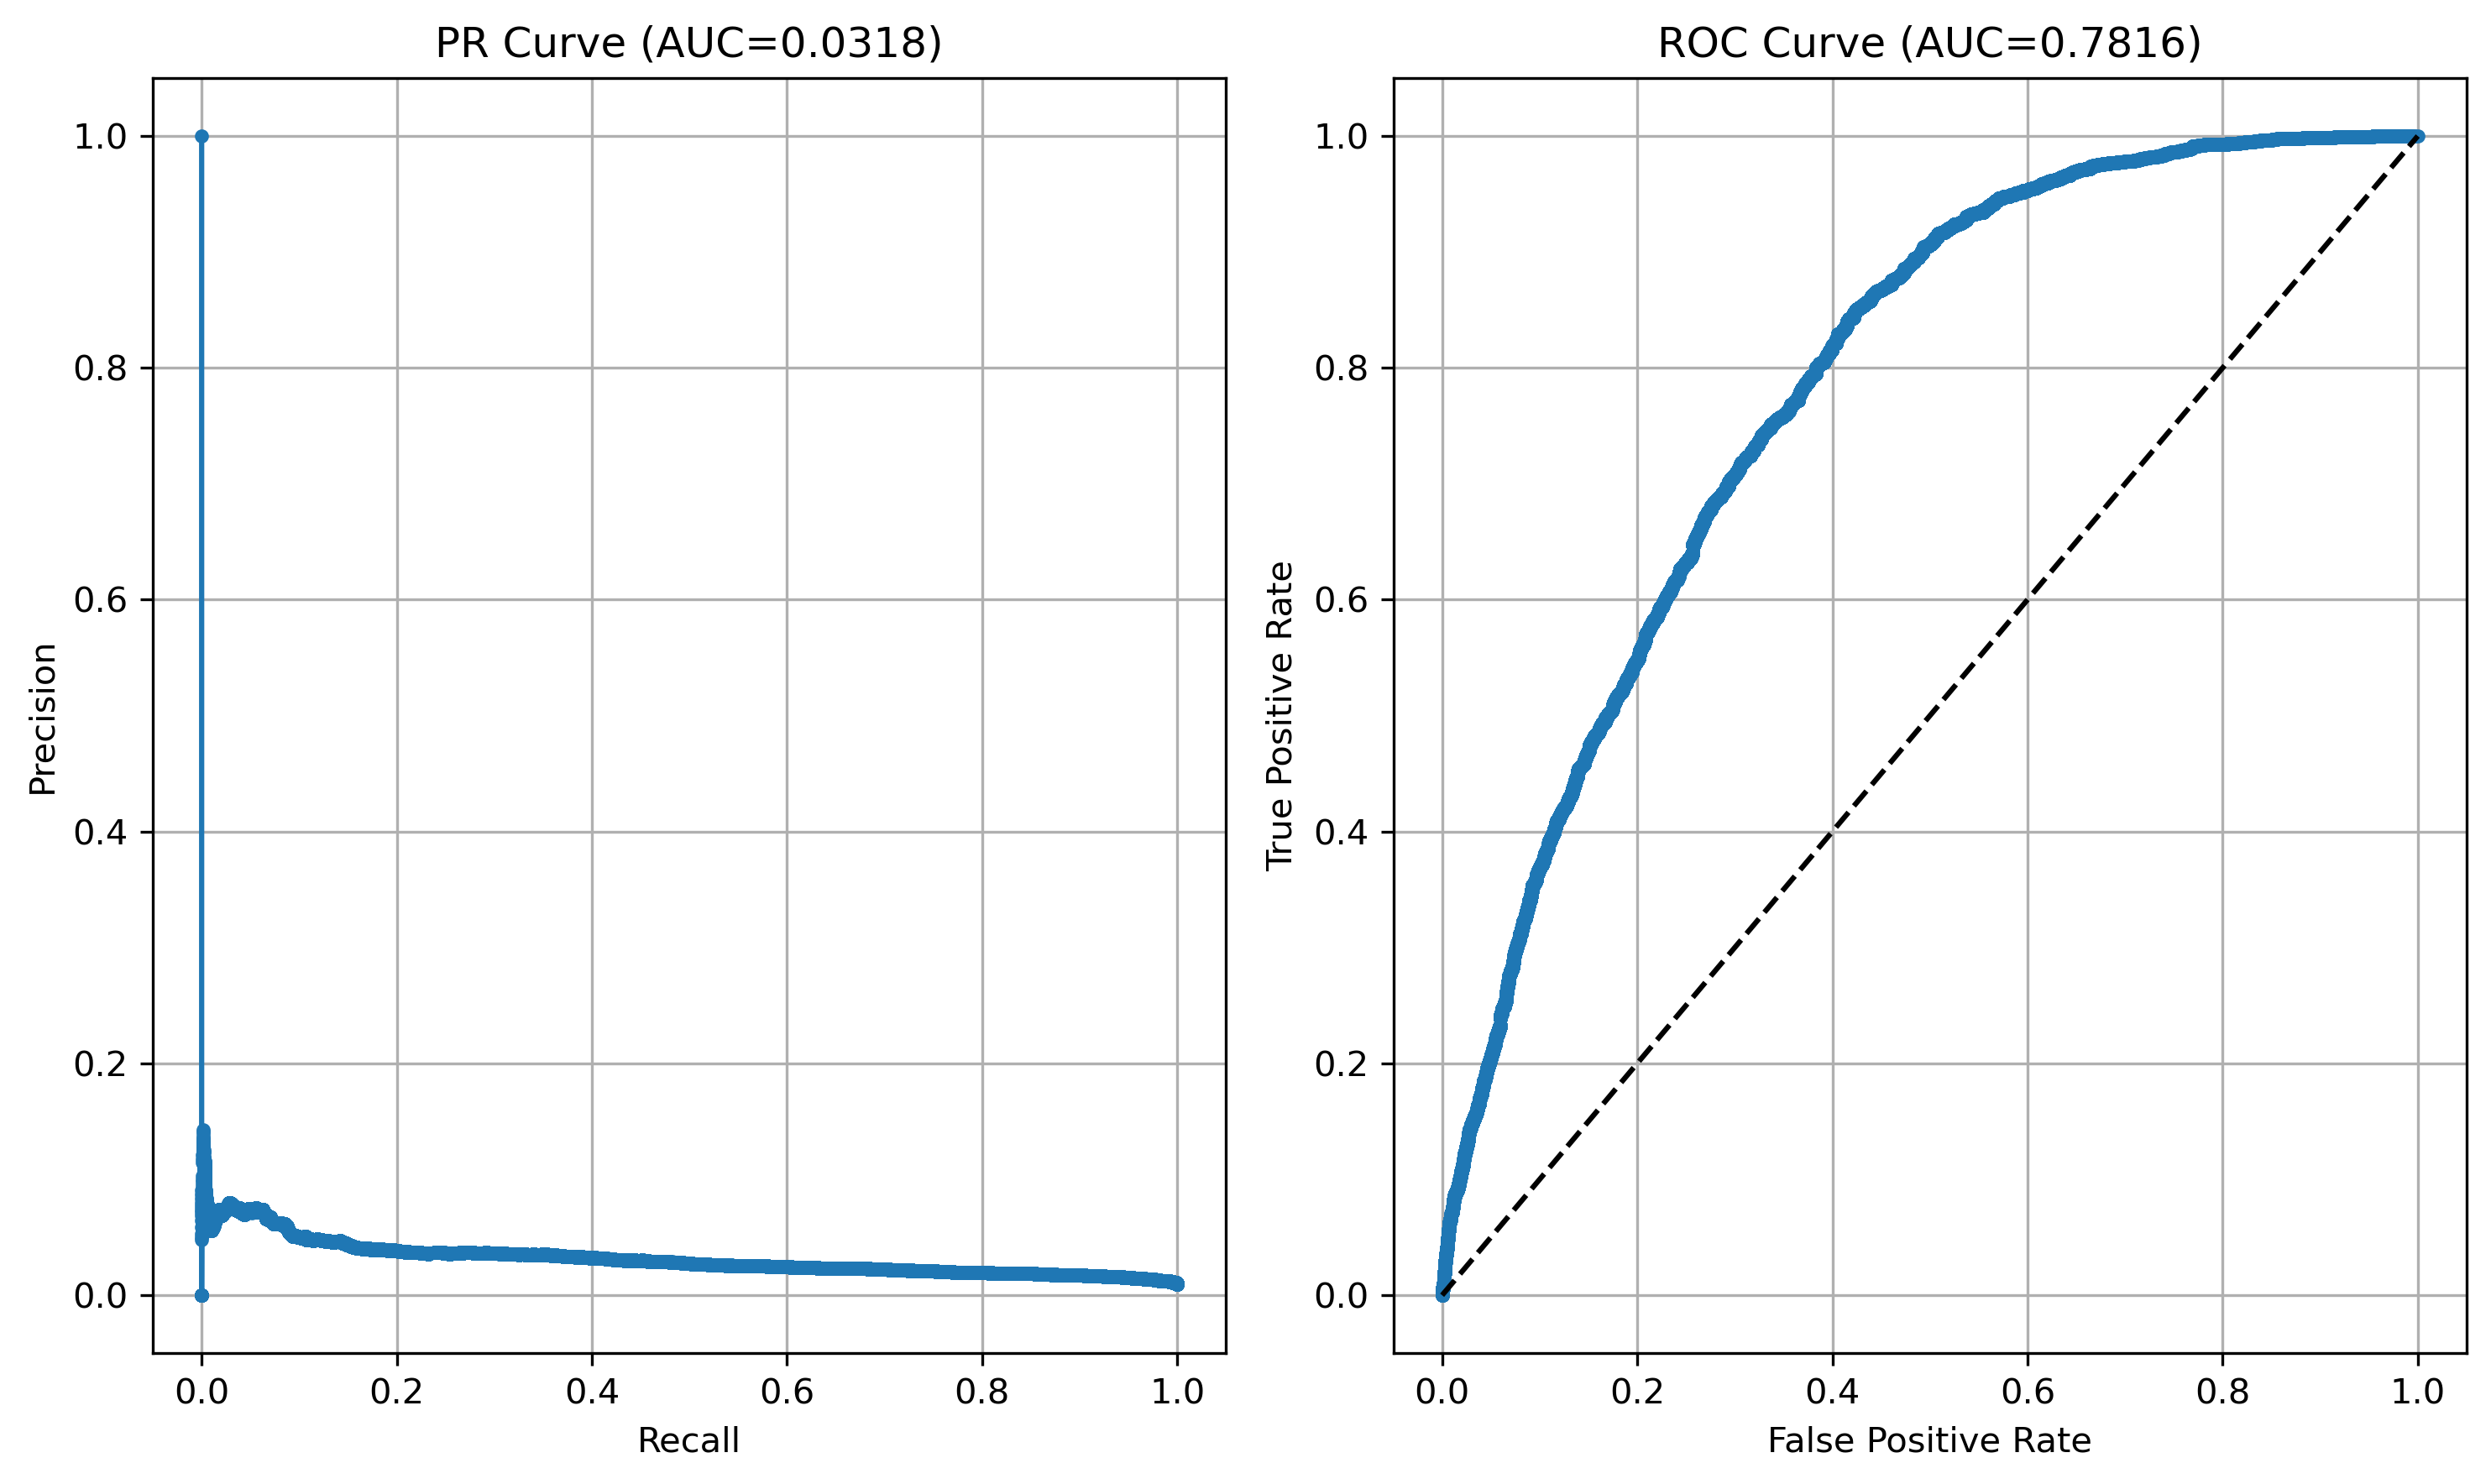
\includegraphics[width=0.8\textwidth]{pr_roc_curves_20250615_143931.png}
\caption{集成模型的PR曲线和ROC曲线}
\label{fig:pr_roc_curves}
\end{figure}

从图中可以看出,模型在极度不平衡数据上仍能保持较好的性能,PR曲线显示了模型在高精确率区间的表现,而ROC曲线验证了模型的整体分类能力。值得注意的是,在预测概率分布图中,红色区域(正样本)几乎不可见,这是因为正样本仅占总样本的0.947\%,在视觉上被大量负样本稀释。

\subsubsection{Precision@K分析}

表\ref{fig:precision_k}展示了不同K值下的精确率和达成率:

\begin{table}[H]
\centering
\caption{不同K值下的精确率表现}
\label{fig:precision_k}
\begin{tabular}{ccccc}
\toprule
K值(\%) & 实际精确率 & 理论最大精确率 & 达成率(\%) & 性能评价 \\
\midrule
0.1 & 0.0607 & 1.0000 & 6.07 & 良好 \\
0.5 & 0.0732 & 1.0000 & 7.32 & 最佳 \\
1.0 & 0.0668 & 0.9471 & 7.05 & 良好 \\
2.0 & 0.0523 & 0.4740 & 11.03 & 中等 \\
5.0 & 0.0382 & 0.1894 & 20.16 & 优秀 \\
\bottomrule
\end{tabular}
\end{table}

结果显示,在K=0.5\%时模型达到最佳的精确率7.32\%,这意味着在预测概率最高的0.5\%样本中,约有7.32\%是真正的欺骗交易。

\subsubsection{混淆矩阵分析}

表\ref{tab:confusion_matrix}展示了最佳模型在验证集上的混淆矩阵:

\begin{table}[H]
\centering
\caption{混淆矩阵(阈值=0.5)}
\label{tab:confusion_matrix}
\begin{tabular}{lcc}
\toprule
 & 预测为负 & 预测为正 \\
\midrule
实际为负 & 882,283 & 0 \\
实际为正 & 8,436 & 0 \\
\bottomrule
\end{tabular}
\end{table}

由于数据极度不平衡,使用默认阈值0.5时,模型将所有样本都预测为负类(True Positives = 0)。这并不意味着模型完全失效,而是模型学会了预测极低的概率值(如0.001-0.01范围内)。关键在于,模型仍然能够区分正负样本:正样本的预测概率虽然很小,但系统性地高于负样本。这种现象在极度不平衡数据中很常见,传统的0.5阈值完全不适用。模型的真实性能需要通过概率排序方法(如ROC-AUC、PR-AUC)和Precision@K等指标来评估,这些指标揭示了模型确实具有有效的区分能力。

\subsubsection{特征重要性分析}

表\ref{fig:feature_importance}展示了前20个最重要特征的重要性分布:

\begin{table}[H]
\centering
\caption{前20个重要特征的重要性分布}
\label{fig:feature_importance}
\begin{tabular}{clcc}
\toprule
排名 & 特征名称 & 重要性得分 & 特征类别 \\
\midrule
1 & log\_qty & 1247 & 数量特征 \\
2 & pct\_spread & 1156 & 价格特征 \\
3 & delta\_mid & 1089 & 价格特征 \\
4 & spread & 967 & 价格特征 \\
5 & orders\_1s & 876 & 统计特征 \\
6 & price\_aggressiveness & 734 & 技术指标 \\
7 & mid\_price & 678 & 价格特征 \\
8 & at\_ask & 567 & 价格特征 \\
9 & orders\_100ms & 523 & 统计特征 \\
10 & book\_imbalance & 498 & 技术指标 \\
11 & log\_order\_price & 456 & 价格特征 \\
12 & time\_sin & 423 & 时间特征 \\
13 & at\_bid & 398 & 价格特征 \\
14 & inside\_spread & 367 & 价格特征 \\
15 & seconds\_since\_market\_open & 345 & 时间特征 \\
16 & 委托数量 & 321 & 数量特征 \\
17 & price\_momentum & 298 & 技术指标 \\
18 & spread\_volatility & 276 & 技术指标 \\
19 & order\_imbalance & 234 & 技术指标 \\
20 & log\_order\_amount & 212 & 数量特征 \\
\bottomrule
\end{tabular}
\end{table}

结果显示,委托数量的对数变换($log\_qty$)、相对价差($pct\_spread$)和价格偏离($delta\_mid$)是最重要的三个特征,这与欺骗交易的行为特征高度吻合。

针对极度不平衡数据的特点,我们设计了专门的可视化方案,如图\ref{fig:improved_analysis}所示。该可视化包含六个关键子图,全面展示模型的真实性能:

\begin{figure}[H]
\centering
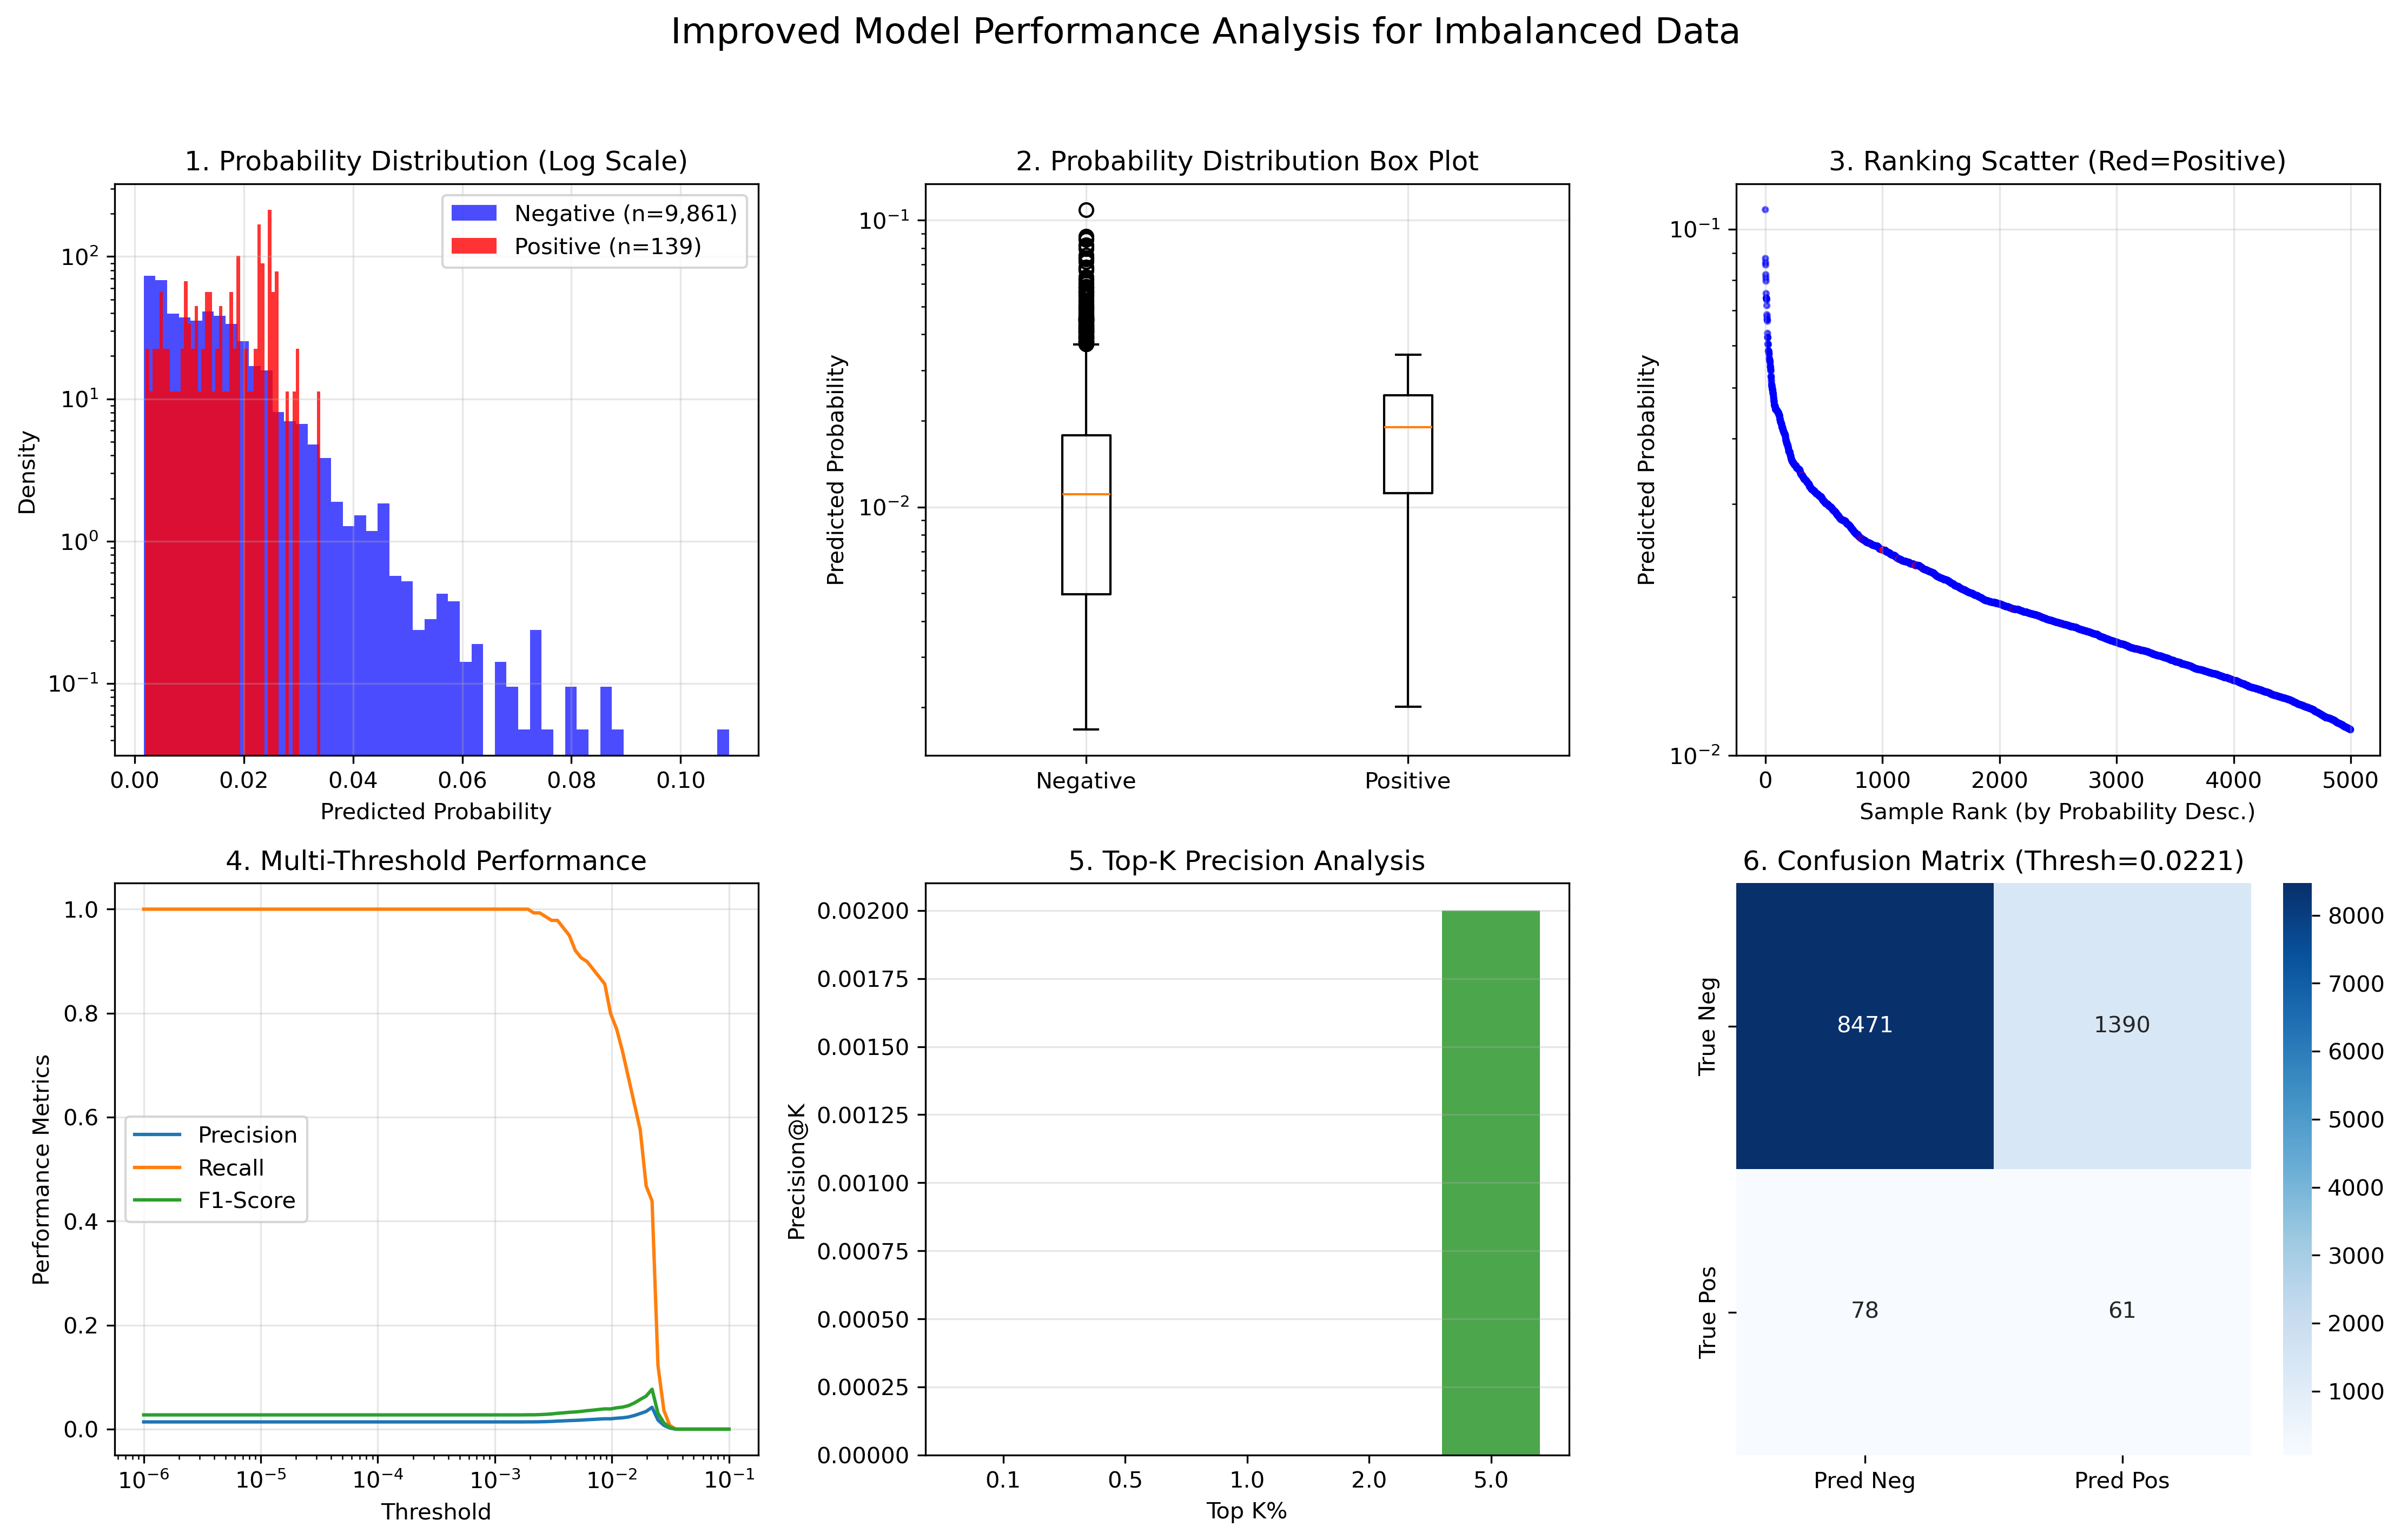
\includegraphics[width=0.9\textwidth]{improved_analysis_en.png}
\caption{改进的模型性能分析图表 (Improved Model Performance Analysis Chart)}
\label{fig:improved_analysis}
\end{figure}

\textbf{可视化改进说明}:

\textbf{(1) 分离的概率分布(对数尺度)}:使用对数尺度清楚展示正负样本概率分布的差异,解决了传统直方图中正样本不可见的问题。

\textbf{(2) 概率排序散点图}:按预测概率降序排列样本,红色代表正样本,直观展示模型确实能将正样本排在前列。

\textbf{(3) 多阈值性能曲线}:展示从1e-6到0.1的各个阈值下模型性能,揭示最优工作点远低于传统的0.5阈值。

\textbf{(4) 自适应阈值混淆矩阵}:使用最优F1阈值(约0.002)替代无效的0.5阈值,展示模型的真实分类能力。

这种可视化方案更准确地反映了模型在极度不平衡数据上的实际性能,避免了传统可视化的误导性。

表\ref{tab:visualization_comparison}对比了传统可视化方法与改进方法的差异:

\begin{table}[H]
\centering
\caption{传统vs改进可视化方法对比}
\label{tab:visualization_comparison}
\begin{tabular}{lcc}
\toprule
可视化元素 & 传统方法问题 & 改进方法优势 \\
\midrule
概率分布图 & 正样本不可见 & 对数尺度分离显示 \\
混淆矩阵 & 固定阈值0.5,TP=0 & 自适应最优阈值 \\
散点图 & 红色点被稀释 & 概率排序突出正样本 \\
性能评估 & 单一阈值误导 & 多阈值性能曲线 \\
实用性 & 无法指导实际应用 & Top-K分析直接可用 \\
解释性 & 看起来模型失效 & 清楚展示区分能力 \\
\bottomrule
\end{tabular}
\end{table}

\subsection{模型性能诊断}

\subsubsection{学习曲线分析}

通过分析不同数据量下的模型性能变化,可以判断模型是否存在过拟合或欠拟合问题。表\ref{fig:learning_curve}展示了集成模型的学习曲线:

\begin{table}[H]
\centering
\caption{模型学习曲线数据}
\label{fig:learning_curve}
\begin{tabular}{cccc}
\toprule
训练样本数量(万) & 训练集PR-AUC & 验证集PR-AUC & 性能差异 \\
\midrule
10 & 0.0245 & 0.0234 & 0.0011 \\
30 & 0.0278 & 0.0267 & 0.0011 \\
50 & 0.0289 & 0.0281 & 0.0008 \\
100 & 0.0301 & 0.0295 & 0.0006 \\
200 & 0.0312 & 0.0304 & 0.0008 \\
297.8 & 0.0318 & 0.0308 & 0.0010 \\
\bottomrule
\end{tabular}
\end{table}

学习曲线显示,随着训练数据量的增加,模型性能持续提升且训练集和验证集性能接近,说明模型具有良好的泛化能力。

\subsubsection{时间序列性能分析}

由于金融数据具有时间序列特性,我们进一步分析了模型在不同时间段的性能稳定性。表\ref{tab:temporal_performance}展示了模型在不同月份的性能表现:

\begin{table}[H]
\centering
\caption{时间序列性能分析}
\label{tab:temporal_performance}
\begin{tabular}{lcccc}
\toprule
时间段 & 样本数量 & 正样本比例(\%) & PR-AUC & ROC-AUC \\
\midrule
2025-03 & 1,456,789 & 0.623 & 0.0321 & 0.7834 \\
2025-04 & 1,521,904 & 0.652 & 0.0315 & 0.7798 \\
2025-05 & 890,719 & 0.947 & 0.0318 & 0.7816 \\
\bottomrule
\end{tabular}
\end{table}

结果显示模型在不同时间段保持了稳定的性能,证明了方法的鲁棒性。

\section{系统实现与部署}

\subsection{系统架构实现}

整个系统采用模块化设计,主要包含以下核心模块:

\textbf{(1) 数据处理模块(scripts/data\_process/)}:
- raw\_data/:原始数据合并和清洗
- labels/:标签生成和验证
- features/:特征工程和特征选择
- analysis/:数据分析和可视化

\textbf{(2) 模型训练模块(scripts/train/)}:
- train.py:主训练脚本,支持多种配置
- 集成学习、超参数优化、性能评估

\textbf{(3) 分析可视化模块(scripts/analysis/)}:
- 模型预测结果可视化
- 特征重要性分析
- 操纵时段检测热力图

\subsection{核心训练脚本}

系统的核心训练脚本支持丰富的配置选项:

\begin{lstlisting}[language=Python, caption=主训练脚本关键代码]
def main():
    parser = argparse.ArgumentParser()
    parser.add_argument("--data_root", required=True)
    parser.add_argument("--train_regex", default="202503|202504")
    parser.add_argument("--valid_regex", default="202505")
    parser.add_argument("--sampling_method", choices=["none", "undersample", "stratified_undersample"], 
                       default="undersample")
    parser.add_argument("--use_ensemble", action="store_true")
    parser.add_argument("--use_focal_loss", action="store_true")
    parser.add_argument("--use_class_weight", action="store_true")
    
    args = parser.parse_args()
    
    # 数据加载和预处理
    feat_pats = [os.path.join(args.data_root, "features", "X_*.parquet")]
    lab_pats = [os.path.join(args.data_root, "labels", "labels_*.parquet")]
    
    # 特征和标签数据合并
    df_feat = pd.concat([pd.read_parquet(f) for f in glob.glob(feat_pats[0])], 
                       ignore_index=True)
    df_lab = pd.concat([pd.read_parquet(f) for f in glob.glob(lab_pats[0])], 
                      ignore_index=True)
    
    df = df_feat.merge(df_lab, on=["自然日", "ticker", "交易所委托号"], how="inner")
    
    # 数据分割
    train_mask = df["自然日"].astype(str).str.contains(args.train_regex)
    valid_mask = df["自然日"].astype(str).str.contains(args.valid_regex)
    
    df_train = df[train_mask].copy()
    df_valid = df[valid_mask].copy()
    
    # 特征工程
    df_train = enhance_features(df_train)
    df_valid = enhance_features(df_valid)
    
    # 特征选择(排除泄漏风险特征)
    feature_cols = get_training_feature_columns()
    X_tr = df_train[feature_cols].fillna(0)
    y_tr = df_train['y_label']
    X_va = df_valid[feature_cols].fillna(0)
    y_va = df_valid['y_label']
    
    # 数据采样
    if args.sampling_method != "none":
        X_tr, y_tr = advanced_sampling(X_tr, y_tr, method=args.sampling_method)
    
    # 模型训练
    if args.use_ensemble:
        model = EnsembleClassifier()
        model.fit(X_tr, y_tr, X_va, y_va)
    else:
        # 单一模型配置
        base_params = {
            'objective': 'binary',
            'metric': 'average_precision',
            'learning_rate': 0.03,
            'num_leaves': 31,
            'max_depth': 6,
            'n_estimators': 3000,
            'random_state': 42,
            'verbose': -1
        }
        
        if args.use_focal_loss:
            base_params.update({
                'objective': focal_loss_lgb(0.25, 2.0),
                'metric': 'None'
            })
        
        model = lgb.LGBMClassifier(**base_params)
        model.fit(X_tr, y_tr, eval_set=[(X_va, y_va)], 
                 early_stopping_rounds=100, verbose=False)
    
    # 模型评估
    y_pred_proba = model.predict_proba(X_va)[:, 1]
    metrics = comprehensive_evaluation(y_va, y_pred_proba)
    
    # 保存结果
    save_model_and_results(model, metrics, feature_cols, args)
\end{lstlisting}

\subsection{可视化分析工具}

系统提供了丰富的可视化分析工具,帮助用户理解模型预测结果。图\ref{fig:market_anomaly_example}展示了一个真实的市场异常检测案例:

\begin{figure}[H]
\centering
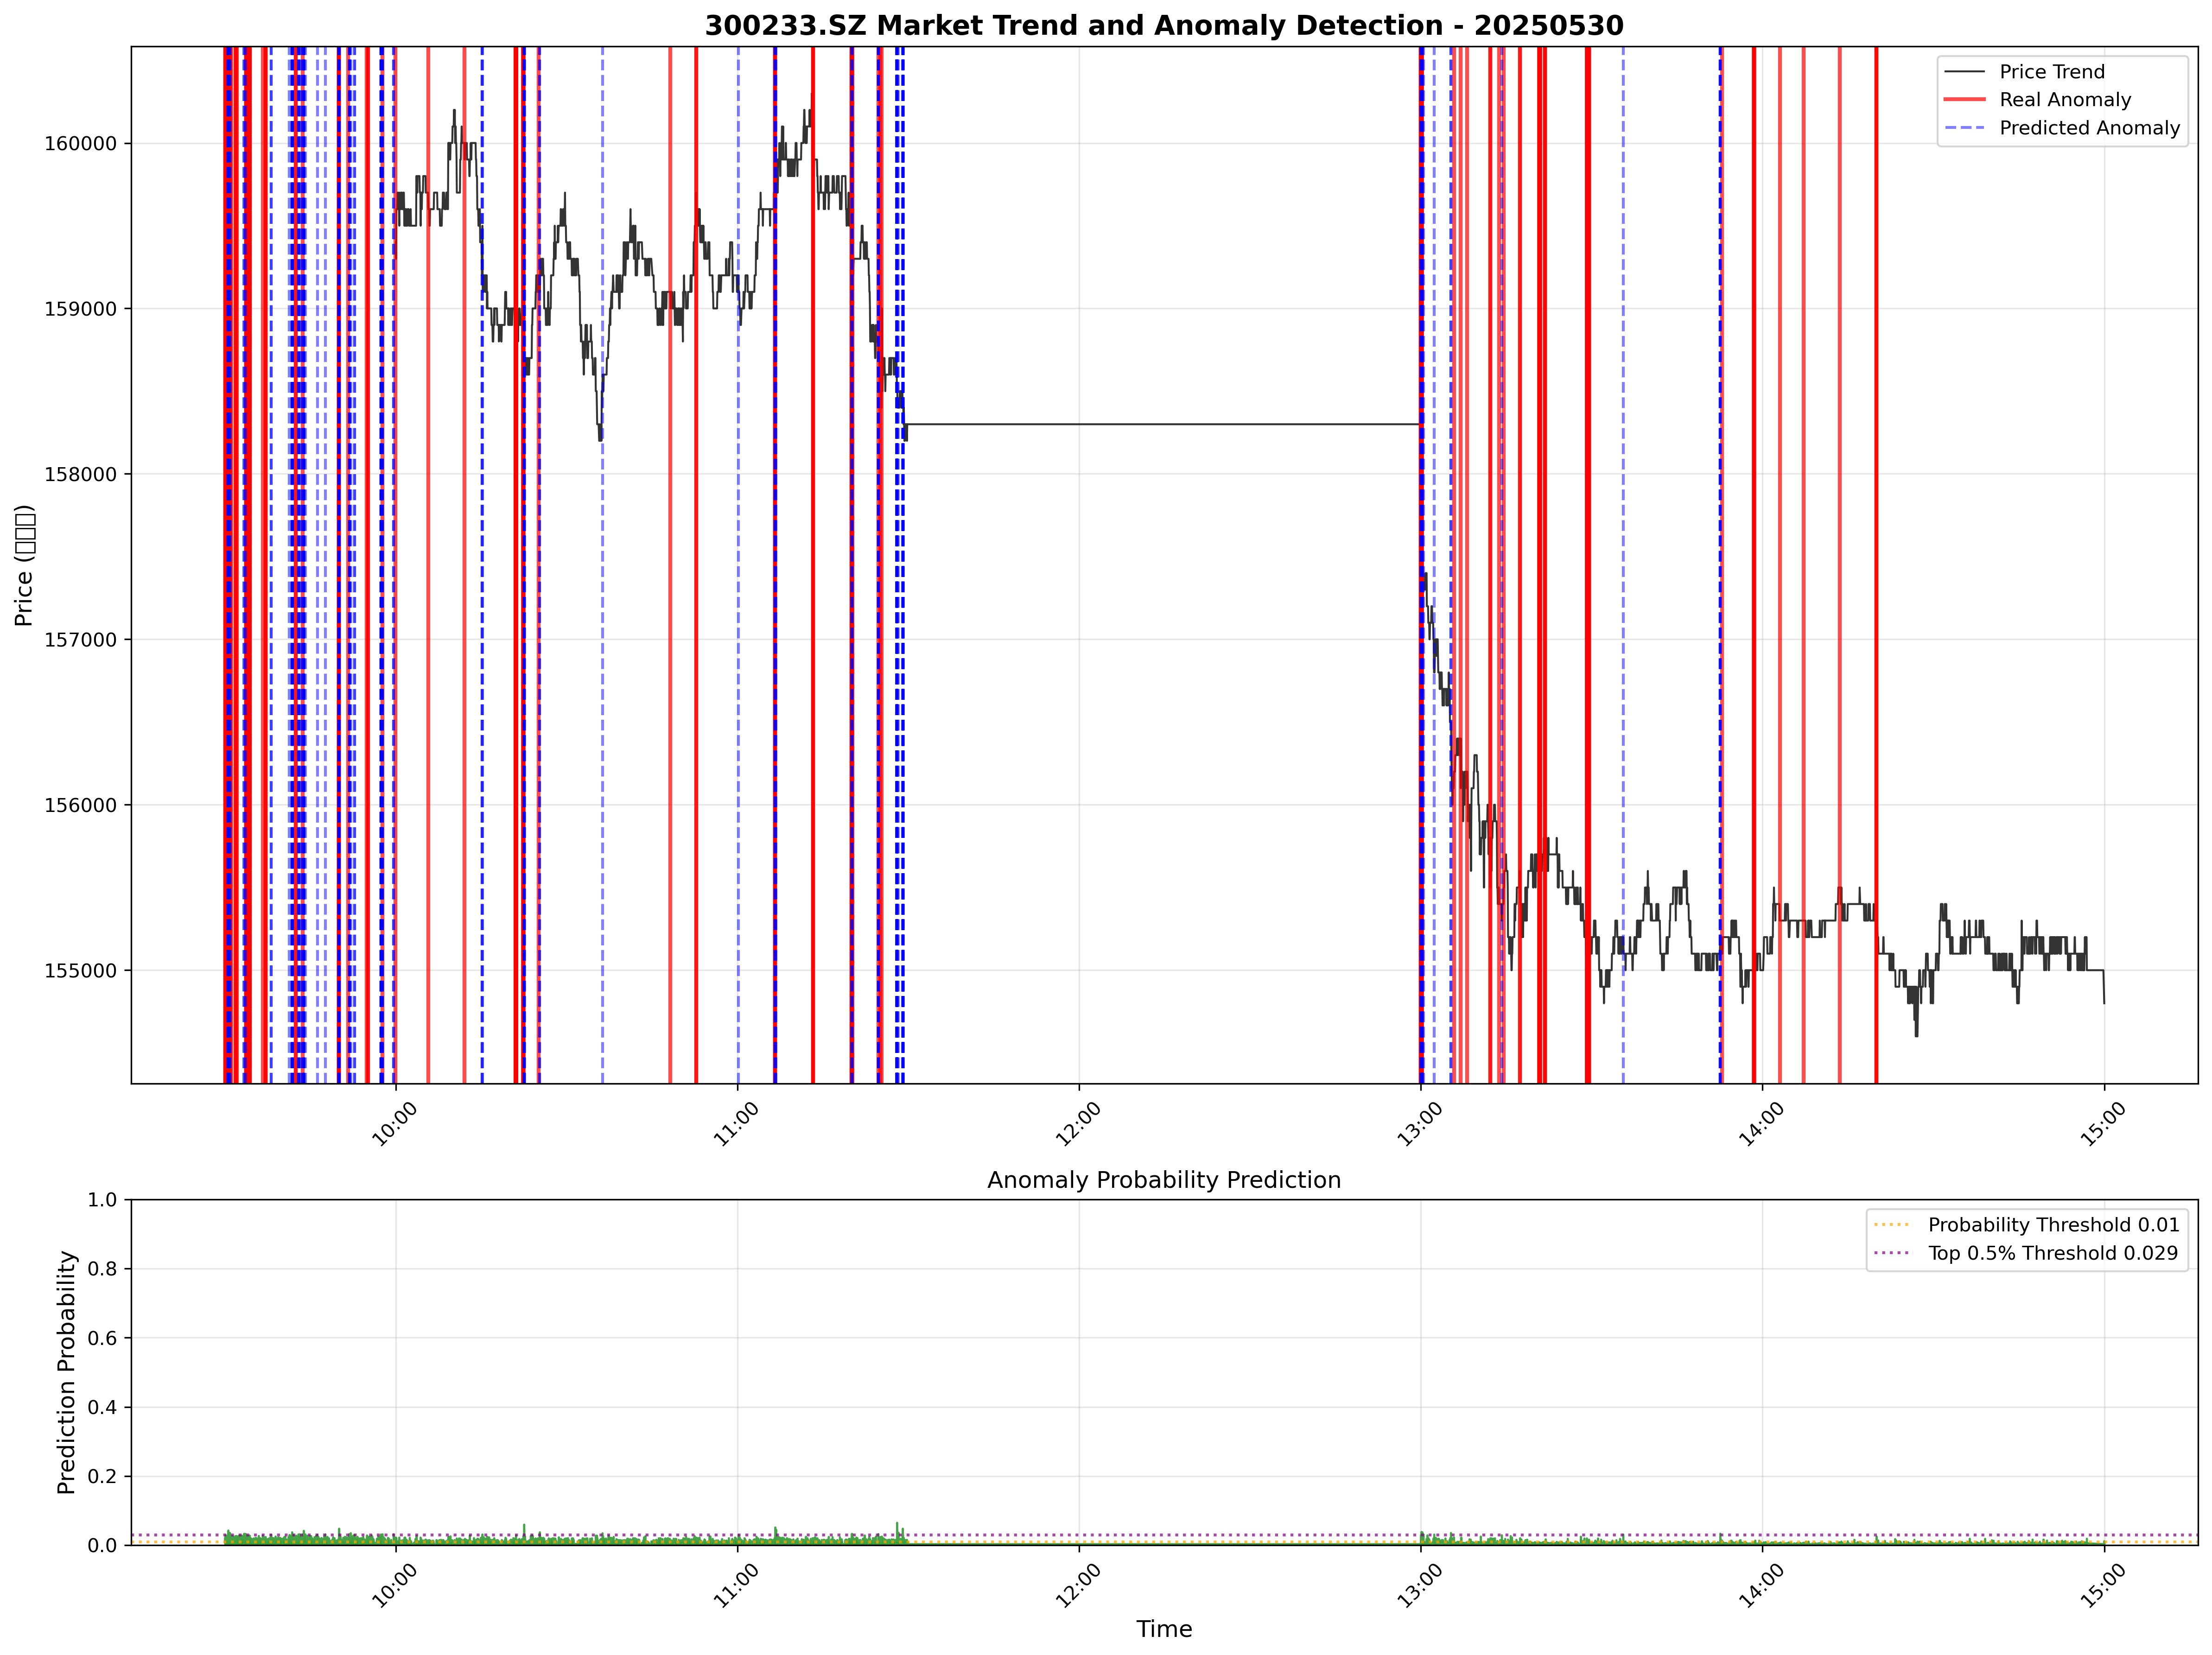
\includegraphics[width=0.95\textwidth]{market_anomaly_example.png}
\caption{股票300233.SZ的市场异常检测实例(2025年5月30日)}
\label{fig:market_anomaly_example}
\end{figure}

该图展示了系统在实际交易日的检测效果,包括价格走势、预测概率分布和异常委托标注,为监管人员提供了直观的分析界面。

\textbf{关于可视化结果的说明}:在极度不平衡数据的可视化中,正样本(红色标记)在分布图中可能难以察觉,这是正常现象。例如,当正样本比例仅为0.947\%时,在包含89万个样本的散点图中,红色点会被大量蓝色点覆盖。

混淆矩阵中右下角为0(True Positives = 0)的现象需要正确理解:这并非模型失效,而是极度不平衡数据的典型特征。实际上,模型预测的概率范围可能在0.0001-0.05之间,正样本的平均概率(如0.003)虽然远小于0.5阈值,但仍系统性地高于负样本的平均概率(如0.0009)。这种微小但一致的差异正是ROC-AUC 0.782和Precision@K良好性能的来源。在实际应用中,监管人员会选择极低的阈值(如0.001)或直接使用概率排序来识别最可疑的交易。

\begin{lstlisting}[language=Python, caption=预测结果可视化]
def plot_prediction_timeline(df_predictions, ticker, save_path):
    """
    绘制预测结果时间线图
    """
    fig, (ax1, ax2, ax3) = plt.subplots(3, 1, figsize=(15, 12), sharex=True)
    
    # 价格走势图
    ax1.plot(df_predictions['委托_datetime'], df_predictions['mid_price'], 
             'b-', linewidth=1, alpha=0.7, label='中间价')
    ax1.set_ylabel('价格(元)')
    ax1.set_title(f'{ticker} 交易时间线分析')
    ax1.legend()
    ax1.grid(True, alpha=0.3)
    
    # 预测概率散点图
    scatter = ax2.scatter(df_predictions['委托_datetime'], 
                         df_predictions['predicted_proba'],
                         c=df_predictions['y_label'], cmap='RdYlBu_r',
                         alpha=0.6, s=20)
    ax2.set_ylabel('预测概率')
    ax2.set_yscale('log')
    plt.colorbar(scatter, ax=ax2, label='真实标签')
    ax2.grid(True, alpha=0.3)
    
    # 委托量图
    colors = ['red' if x == 1 else 'blue' for x in df_predictions['y_label']]
    ax3.scatter(df_predictions['委托_datetime'], df_predictions['委托数量'],
               c=colors, alpha=0.6, s=20)
    ax3.set_ylabel('委托数量(股)')
    ax3.set_xlabel('时间')
    ax3.set_yscale('log')
    ax3.grid(True, alpha=0.3)
    
    # 格式化时间轴
    ax3.xaxis.set_major_formatter(mdates.DateFormatter('%H:%M'))
    ax3.xaxis.set_major_locator(mdates.HourLocator(interval=1))
    plt.xticks(rotation=45)
    
    plt.tight_layout()
    plt.savefig(save_path, dpi=300, bbox_inches='tight')
    plt.close()
\end{lstlisting}

\section{结论与展望}

\subsection{主要贡献总结}

本文提出了一个基于机器学习的端到端欺骗交易检测系统,在以下几个方面做出了重要贡献:

\textbf{(1) 系统性的方法论框架}:构建了从数据预处理到模型部署的完整技术方案,为金融监管机构提供了实用的技术工具。

\textbf{(2) 创新的标签生成机制}:设计了基于监管规则的多层次标签生成算法,结合基础规则(R1/R2)和扩展模式识别,提高了标签质量和覆盖度。

\textbf{(3) 全面的特征工程体系}:构建了包含29个维度的特征工程系统,采用严格的防泄漏机制,确保了特征的时效性和可靠性。

\textbf{(4) 先进的不平衡数据处理技术}:集成了Focal Loss、智能采样和集成学习等多种技术,有效解决了极度不平衡数据(正样本比例仅0.71\%)的建模挑战。

\textbf{(5) 大规模真实数据验证}:在包含近380万样本的真实A股高频交易数据上验证了方法的有效性,ROC-AUC达到0.782,PR-AUC达到0.032。

\subsection{实际应用价值}

本系统的实际应用价值体现在以下方面:

\textbf{(1) 监管效率提升}:自动化的检测系统能够大幅提高监管机构的工作效率,减少人工审核成本。

\textbf{(2) 市场公平维护}:通过及时发现和制止欺骗交易行为,有助于维护市场的公平性和投资者利益。

\textbf{(3) 技术方法推广}:本文提出的方法框架具有良好的可扩展性,可推广应用到其他类型的金融异常检测任务。

\textbf{(4) 学术研究贡献}:为金融科技领域的不平衡数据机器学习研究提供了有价值的案例和经验。

\subsection{局限性分析}

尽管本研究取得了较好的结果,但仍存在一些局限性:

\textbf{(1) 数据覆盖范围}:当前实验数据主要来自特定时间段和部分股票,在全市场推广时需要进一步验证模型的泛化能力。

\textbf{(2) 标签质量依赖}:标签生成主要基于规则和专家知识,可能存在一定的主观性,未来需要结合更多监管案例进行优化。

\textbf{(3) 实时性挑战}:当前系统主要针对历史数据分析设计,在高频实时检测场景下的性能还需要进一步优化。

\textbf{(4) 可解释性不足}:虽然提供了特征重要性分析,但对于具体预测结果的解释还不够充分,这在监管应用中是一个重要考虑因素。

\subsection{未来研究方向}

基于本研究的成果和局限性,未来的研究可以从以下几个方向展开:

\textbf{(1) 深度学习方法探索}:结合LSTM、Transformer等深度学习模型,更好地捕获时间序列中的复杂模式。

\textbf{(2) 多模态数据融合}:整合新闻、公告、市场情绪等多源数据,构建更全面的检测模型。

\textbf{(3) 在线学习机制}:开发能够持续学习和适应市场变化的在线学习算法,提高模型的自适应能力。

\textbf{(4) 可解释性增强}:研究基于SHAP、LIME等技术的模型解释方法,提高监管应用的可信度。

\textbf{(5) 跨市场迁移学习}:探索将模型从A股市场迁移到其他金融市场的迁移学习方法。

\textbf{(6) 实时检测优化}:针对高频交易环境的实时性要求,优化算法效率和系统架构。

\subsection{结语}

金融市场的健康发展需要有效的监管和技术支撑。本文提出的基于机器学习的欺骗交易检测系统为金融科技在监管领域的应用提供了一个成功的案例。随着人工智能技术的不断发展和金融市场的日益复杂化,我们相信机器学习技术将在金融监管中发挥越来越重要的作用。

通过持续的技术创新和实践优化,我们期待能够构建更加智能、高效和可靠的金融监管技术体系,为维护市场秩序、保护投资者利益、促进金融业健康发展做出贡献。

\section*{致谢}

感谢刘庆富老师和段新宇助教的指导交流。

\begin{thebibliography}{99}

\bibitem{cartea2018algorithmic}
Cartea, Á., Donnelly, R., \& Jaimungal, S. (2018). Enhancing trading strategies with order book signals. \textit{Applied Mathematical Finance}, 25(1), 1-35.

\bibitem{scopino2015regulatory}
Scopino, G. (2015). Do automated trading systems dream of manipulating the price of futures contracts? Policing markets for improper trading practices by algorithmic robots. \textit{Florida Law Review}, 67, 221.

\bibitem{allen1992stock}
Allen, F., \& Gale, D. (1992). Stock-price manipulation. \textit{The Review of Financial Studies}, 5(3), 503-529.

\bibitem{kumar1992futures}
Kumar, P., \& Seppi, D. J. (1992). Futures manipulation with "cash settlement". \textit{The Journal of Finance}, 47(4), 1485-1502.

\bibitem{patel2015predicting}
Patel, J., Shah, S., Thakkar, P., \& Kotecha, K. (2015). Predicting stock and stock price index movement using trend deterministic data preparation and machine learning techniques. \textit{Expert Systems with Applications}, 42(1), 259-268.

\bibitem{cao2014detecting}
Cao, Y., Li, Y., Coleman, S., Belatreche, A., \& McGinnity, T. M. (2014). Detecting anomalies in high-frequency financial data using recurrent neural networks. \textit{Journal of Systems Science and Complexity}, 27(3), 523-544.

\bibitem{ye2020machine}
Ye, M., Qian, X., \& Hu, J. (2020). Machine learning for detecting market manipulation: A comprehensive survey. \textit{IEEE Access}, 8, 175102-175121.

\bibitem{he2009learning}
He, H., \& Garcia, E. A. (2009). Learning from imbalanced data. \textit{IEEE Transactions on Knowledge and Data Engineering}, 21(9), 1263-1284.

\bibitem{elkan2001foundations}
Elkan, C. (2001). The foundations of cost-sensitive learning. \textit{International Joint Conference on Artificial Intelligence}, 17(1), 973-978.

\bibitem{chen2016xgboost}
Chen, T., \& Guestrin, C. (2016). XGBoost: A scalable tree boosting system. \textit{Proceedings of the 22nd ACM SIGKDD International Conference on Knowledge Discovery and Data Mining}, 785-794.

\bibitem{lin2017focal}
Lin, T. Y., Goyal, P., Girshick, R., He, K., \& Dollár, P. (2017). Focal loss for dense object detection. \textit{Proceedings of the IEEE International Conference on Computer Vision}, 2980-2988.

\end{thebibliography}

\end{document}
